\chapter{Estado del arte}
\label{cap:estadoDelArte}
En esta sección nos centraremos en explicar el ámbito en el que se enmarca nuestro proyecto. Inicialmente en la Sección \ref{cap:adaptacion} definiremos el concepto de adaptación curricular, explicaremos en detalle los posibles tipos y añadiremos ejemplos de adaptaciones según las diferentes necesidades que pueden tener los estudiantes. En la Sección \ref{sec:herramientasexistentes}  se expondrán las herramientas existentes para la adaptación curricular, entre las que se encuentra explicada AdaptaMaterialEscolar 1.0, la herramienta que servirá de base para nuestro trabajo.

\section{Adaptación curricular}\label{cap:adaptacion}
Para poder comprender la adaptación curricular, inicialmente se debe definir la palabra currículum. En el artículo 2 del BOE (\citeyear[p.5]{BOE2}) se define el currículum como \textit{``regulación de los elementos que determinan los procesos de enseñanza y aprendizaje para cada una de las enseñanzas y etapas educativas.}'' Es decir, el currículum especifica los contenidos, materiales y recursos que deben presentar y administrar las instituciones educativas de todos los niveles.

En nuestro sistema educativo, aceptar la diversidad del alumnado y la individualidad de cada uno de ellos constituye la base del quehacer de los docentes. Los profesores deben modificar el currículum y el programa de aula con el fin de mejorar el desarrollo del aprendizaje. Para poder realizar dicha actividad, el profesorado deberá detectar, evaluar y valorar al alumno, y a los elementos curriculares y del entorno. Tras llevar a cabo lo anterior, el profesorado debe realizar las adaptaciones curriculares necesarias para lograr una mejora en el desarrollo personal y social del alumno \citep*{adaptacionIntro}.

En el artículo 7 del BOE (\citeyear[p.7]{BOE}) se define la adaptación curricular como \textit{``la medida de modificación de los elementos del currículo a fin de dar respuesta a las necesidades del alumnado. En todo caso, la adaptación tendrá como referente los objetivos y las competencias básicas del currículo que corresponda.''} Es decir, la adaptación curricular es cualquier adaptación del currículo realizado para aquellos estudiantes cuyas necesidades no se encuentran cubiertas por el currículo ordinario y, por tanto, no pueden acceder a él de la misma manera que sus compañeros.

Para poder aplicar la adaptación curricular a un alumno se debe precisar el tipo de adaptación en función de sus necesidades, de manera que pueda alcanzar los objetivos propuestos. Para ello, definimos en las siguientes subsecciones los tipos de adaptaciones más utilizadas \citep*{adaptacionUNED}, enfocándonos tanto en las adaptaciones curriculares de acceso al currículum como en las adaptaciones curriculares individualizadas.

\subsection{Adaptaciones de acceso al currículum}
\label{adaptacionesAcceso}
Las adaptaciones de acceso permiten al alumno con necesidades educativas especiales acceder a los diferentes componentes del currículum. No implica una adaptación del currículum sino una adaptación en los recursos materiales, espaciales o de comunicación para que los alumnos con necesidades educativas especiales puedan desarrollar el currículum. Dicha adaptación puede tomar a su vez diferentes tipos: espacial, material o de comunicación. En las siguientes subsecciones explicaremos en detalle cada uno de estos tipos de adaptación.

\subsubsection{Acceso espacial}
Hace referencia a las adaptaciones en relación con el espacio ya sea el aula o el colegio. Destacan las siguientes:
\begin{itemize}
    \item \textbf{Adaptación en la sonorización del aula:} Las aulas deben tener un cierto nivel de volumen adecuado, sin que haya ruidos continuos, sin eco, etc. Dichas clases son especialmente adecuadas para estudiantes que tienen impedimentos auditivos o visuales o que requieren, por su propia condición especial, un entorno con pocos estímulos auditivos que les distraiga.
    \item \textbf{Adaptación en la iluminación del aula:} Las aulas bien iluminadas requieren que estas no tengan sombras, deben poseer ventanales que suministren luz natural o en su lugar luz artificial que proporcione una iluminación óptima. Estos requisitos son necesarios para los estudiantes con discapacidades sensoriales, como por ejemplo, las personas que presentan visión monocular.
    \item \textbf{Adaptación en el espacio físico:} Es todo aquello relacionado con la ausencia de barreras arquitectónicas:  braille en las puertas, ascensores, pasamanos, remate de las escaleras rugoso, etc. En esta sección también se encuentran los aspectos relacionados con la ubicación del aula (sin escaleras, lugares poco ruidosos) y con la disposición del estudiante dentro del aula (al lado de un enchufe, del profesor, de la puerta, etc.)
\end{itemize}

\subsubsection{Acceso material}
Este tipo de adaptación incluye dos tipos, los materiales adaptados y los materiales específicos:
\begin{itemize}
    \item \textbf{Materiales adaptados:} Se refieren a materiales que se usan habitualmente, y que se adaptan para un uso apropiado por parte de los alumnos con necesidades especiales. Ejemplos de ello sería plastificar un libro o hacer dibujos con relieve.
    \item \textbf{Materiales específicos:} A los alumnos con necesidades especiales se les proporcionan materiales específicos con el fin de superar las dificultades relacionadas con los elementos del aula. Por ejemplo, incluir sillas especiales para personas con discapacidad motora, comunicadores electrónicos con salidas de voz o escritas o máquinas de Braille para alumnos con discapacidad visual.
\end{itemize}

\subsubsection{Acceso de comunicación}
Algunos alumnos son incapaces de comprender o expresarse por medio del lenguaje oral, o su nivel no es suficiente para poder comunicarse correctamente. Dichos alumnos requieren estudiar y usar códigos de comunicación suplementarios al lenguaje oral, o alguna alternativa al mismo. Aprender dichos códigos de comunicación facilitará el acceso a los elementos curriculares ordinarios y les concederá una herramienta imprescindible tanto para el desarrollo de algunas competencias y aprendizajes de diferentes contenidos, como para relacionarse y comunicarse con el resto de personas. De esta manera, podemos destacar los siguientes sistemas que mejoran el acceso a la comunicación:
\begin{itemize}
    \item \textbf{Sistemas alternativos a la comunicación:} Estos sistemas no requieren del lenguaje oral para su utilización. Ejemplo de estos procedimientos son los símbolos pictográficos para la comunicación, la lengua de signos española, etc.

    \item \textbf{Sistemas complementarios a la comunicación:} No sustituyen al lenguaje oral, se encargan de reducir los problemas de comunicación y apoyar el acceso al lenguaje oral. Destacan la palabra complementada (sistema complementario de lectura labial) y la comunicación bimodal (es un sistema de comunicación que utiliza el habla y los signos al mismo tiempo).
\end{itemize}

\subsection{Adaptaciones curriculares individualizadas}

Las adaptaciones curriculares individualizadas son modificaciones curriculares que se realizan para satisfacer las necesidades de un alumno en concreto. En las siguientes subsecciones explicamos cada una de ellas en detalle.

\subsubsection{Adaptaciones curriculares significativas}
Según el el artículo 8 del BOE (\citeyear[p. 7]{BOE}), \textit{``una adaptación curricular será significativa cuando la modificación de los elementos del currículo afecten al grado de consecución de los objetivos, los contenidos y los aprendizajes imprescindibles que determinan las competencias básicas en la etapa, ciclo, grado, curso o nivel correspondiente.''} Es decir, son los ajustes que se realizan en el contenido del currículum. Para su elaboración e implementación se debe considerar los siguientes enfoques:
\begin{itemize}
    \item Inclusión. Se introducen elementos curriculares no presentes en el currículo. Puede incorporar objetivos, contenidos, criterios de evaluación, etc; conforme a las necesidades del alumno.
    \item Reformulación. Esta adaptación modifica sustancialmente los elementos del currículum en relación con su Programa de Aula (concreción del currículum oficial que se realizará día a día en el aula). Un ejemplo de reformulación sería el siguiente, un alumno de primero de Educación Secuendaria Obligatoria (ESO) debería pasar al siguiente curso sabiendo la jerarquía y la manipulación de las operaciones con los números naturales. En el caso de que un alumno tenga dificultades con el contenido de las operaciones con los números naturales, el profesor podría enseñar al alumno a manipular las operaciones básicas, pero no aprendería la jerarquía de esta.

    \item Temporalización fuera de ciclo. Los alumnos con ritmo de aprendizaje lento con respecto a sus compañeros tendrán la oportunidad de conseguir los objetivos en otro ciclo posterior, posponiendo a otras etapas algunos elementos curriculares.
    \item Eliminación. Este tipo de adaptación es la más significativa. Inicialmente se deben eliminar contenidos, a continuación, criterios de evaluación y objetivos, y finalmente se propondrá quitar material.
\end{itemize}

\subsubsection{Adaptaciones curriculares no significativas}
Son adaptaciones que no modifican sustancialmente el contenido del currículo oficial, es decir, se adapta la metodología, las actividades, los tiempos, las técnicas e instrumentos de evaluación. Para su elaboración se debe considerar los siguientes elementos:
\begin{itemize}
    \item Evaluación: Se ajusta la manera de evaluar a las necesidades del alumno. Ejemplo de ello es cuando un alumno con escayola no puede realizar un examen escrito por lo que se le adapta la forma de evaluar realizando un examen oral.
    \item Metodología: Aquí se hace mención a cómo se enseña, es decir, a la forma de transmitir el aprendizaje. El desarrollo de la enseñanza-aprendizaje ha de ser activo, partiendo desde las necesidades del alumno. Además, ha de ser creativo, cooperativo y buscar una opción distinta al método tradicional de trabajo. Por ejemplo, reducir y fragmentar las actividades, proporcionando contenidos estructurados y organizados, combinar trabajos más estimulantes con otros menos motivadores, etc.
    \item Priorización de objetivos o contenidos: Dentro de la planificación se podría dar más valor a unos contenidos que a otros.
    \item Temporalización de contenidos u objetivos: Permitir más tiempo para alcanzar algunos de los contenidos pero respetando el ciclo.
\end{itemize}

\subsection{Ejemplificación de algunas adaptaciones curriculares asociadas a diferentes necesidades }

En esta sección se enumerarán algunos ejemplos de adaptaciones curriculares de acceso al currículum y de adaptaciones curriculares individualizadas asociadas a distintas necesidades según la clasificación de \citep*{adaptacionUNED}.

La discapacidad motora es un grupo de alteraciones que se producen como consecuencia de diversas anomalías en los sistemas que forman el movimiento (\citeauthor{disMotora}). Este tipo de discapacidad requiere  adaptaciones de acceso tales como rampas, pasamanos, suelos antideslizantes, etc. En relación con las adaptaciones significativas atañen sobre todo al área de Educación Física, Música o Plástica ya que en estas asignaturas se precisa del manejo de instrumentos. Por ejemplo, en el área de Educación Física se realizarán ejercicios en los cuales el alumno utilizará los músculos que presenten una mayor funcionalidad, con el fin de mejorar la capacidad de respuesta. Con respecto a las adaptaciones no significativas se debe adaptar la forma de evaluar ya que se debe tener en cuenta su movilidad. Un ejemplo de ello sería realizar los exámenes de forma oral.

La discapacidad auditiva es la pérdida parcial o completa de la audición, supone la sustitución del lenguaje oral por otras vías como la visual (\citeauthor{disAuditiva}). Con respecto a las adaptaciones de acceso, el alumno se debe encontrar en una zona del aula en la que no haya muchas sombras ya que la adquisición de conocimientos se realiza por vía visual. Por otro lado, los alumnos con una pérdida parcial de la audición necesitan de un ambiente poco ruidoso. En relación con las adaptaciones curriculares significativas, los profesores deberán trabajar de forma conjunta con especialistas en audición y lenguaje para que el alumno logre alcanzar los objetivos conectados con el lenguaje oral. En cuanto a las adaptaciones curriculares no significativas, hay que tener en cuenta la manera de evaluar (a través de lengua de signos, evaluaciones objetivas o de respuesta cortas), además de la forma de hablar al alumno, ya que esta debe ser de un modo claro, sin gesticular excesivamente, etc.

La discapacidad intelectual es una condición que se caracteriza por limitaciones significativas tanto en el funcionamiento intelectual como en el comportamiento adaptativo (\citeauthor{disIntelectual}). En este tipo de discapacidad no es muy relevante la adaptación de acceso, pero podemos destacar el posicionamiento del alumno en el aula, de manera que se encuentre en una zona donde no tenga muchas distracciones. Las adaptaciones curriculares significativas se aplicarán en función de su nivel de competencia curricular. En relación con las adaptaciones curriculares no significativas se centrarán en la metodología, como por ejemplo programar actividades que permitan la experimentación (manipulación).

El espectro autista hace referencia a una variedad de trastornos del neurodesarrollo que se caracterizan por déficits sociales y de comunicación, y conductas restringidas y repetitivas (\citeauthor{espectroAutista}). En relación con las adaptaciones de acceso al espacio se precisa no realizar grandes cambios en la disposición del mobiliario. También destacamos las adaptaciones de comunicación, ya que las personas autistas se caracterizan por la ausencia de comunicación según el nivel. Para ayudar a romper la barrera de la comunicación lo que realizan es asociar palabras con gestos e impulsar un refuerzo positivo. En cuanto a las adaptaciones curriculares significativas, se debe introducir o priorizar el contenido en lo que respecta a la  comunicación o rediseñar los objetivos o elementos que no puedan alcanzar. Las adaptaciones curriculares no significativas se centran en la metodología. Las actividades deben de ser consistentes, con una estructura y organización claras.

Para las altas capacidades intelectuales no se requiere de adaptaciones de acceso ya que  este tipo de alumnos no tienen dificultades para acceder al currículum. Con respecto a las adaptaciones curriculares significativas lo que deberían realizar los profesores es ampliar el currículum añadiendo objetivos y contenidos. Las adaptaciones curriculares no significativas hacen hincapié en la metodología, por ejemplo, haciendo actividades de ampliación.

\section{Herramientas existentes para adaptaciones curriculares}
\label{sec:herramientasexistentes}
Para llevar a cabo el proyecto y poder ofrecer a nuestros usuarios finales una herramienta de calidad, hemos investigado herramientas existentes que faciliten la adaptación curricular para ayudarnos a diseñar las funcionalidades de AdaptaMaterialEscolar 2.0. A continuación, se explica el funcionamiento básico de algunas de las herramientas existentes que hemos investigado y se explica en detalle AdaptaMaterialEscolar 1.0.

\subsection{SymWriter}
SymWriter\footnote{\url{https://www.widgit.com/es/support/index.htm}} es un procesador de texto que traduce las palabras a pictogramas a medida que se escriben, lo que facilita el acceso a vocabulario nuevo o complejo. También puede ayudar a profesores a crear textos basados en símbolos para potenciar la comprensión visual, entre otras cosas. Además de la traducción automática de palabras a pictogramas, ofrece una función de apoyo auditivo, para que el alumno pueda escuchar las frases del documento o archivos de sonido proporcionados por el profesor. También ofrece un corrector ortográfico con soporte para símbolos y permite añadir imágenes. A medida que se escribe el texto, aparecen los pictogramas encima de las palabras. Estos pictogramas luego se pueden cambiar por otros o por una imagen propia. En la Figura \ref{fig:SymWriter} se muestra la interfaz, y se puede ver como aparecen los pictogramas encima de las palabras y las opciones de los pictogramas en el panel de la derecha. Esta herramienta ofrece una versión de prueba de 21 días, pero al acabarse será necesario adquirir la versión completa\footnote{\url{https://qinera.com/es/software-para-la-comunicacion-y-lectoescritura/132-communicate-symwriter.html}} para poder seguir usándola.

\begin{figure}[ht!]
    \centering
    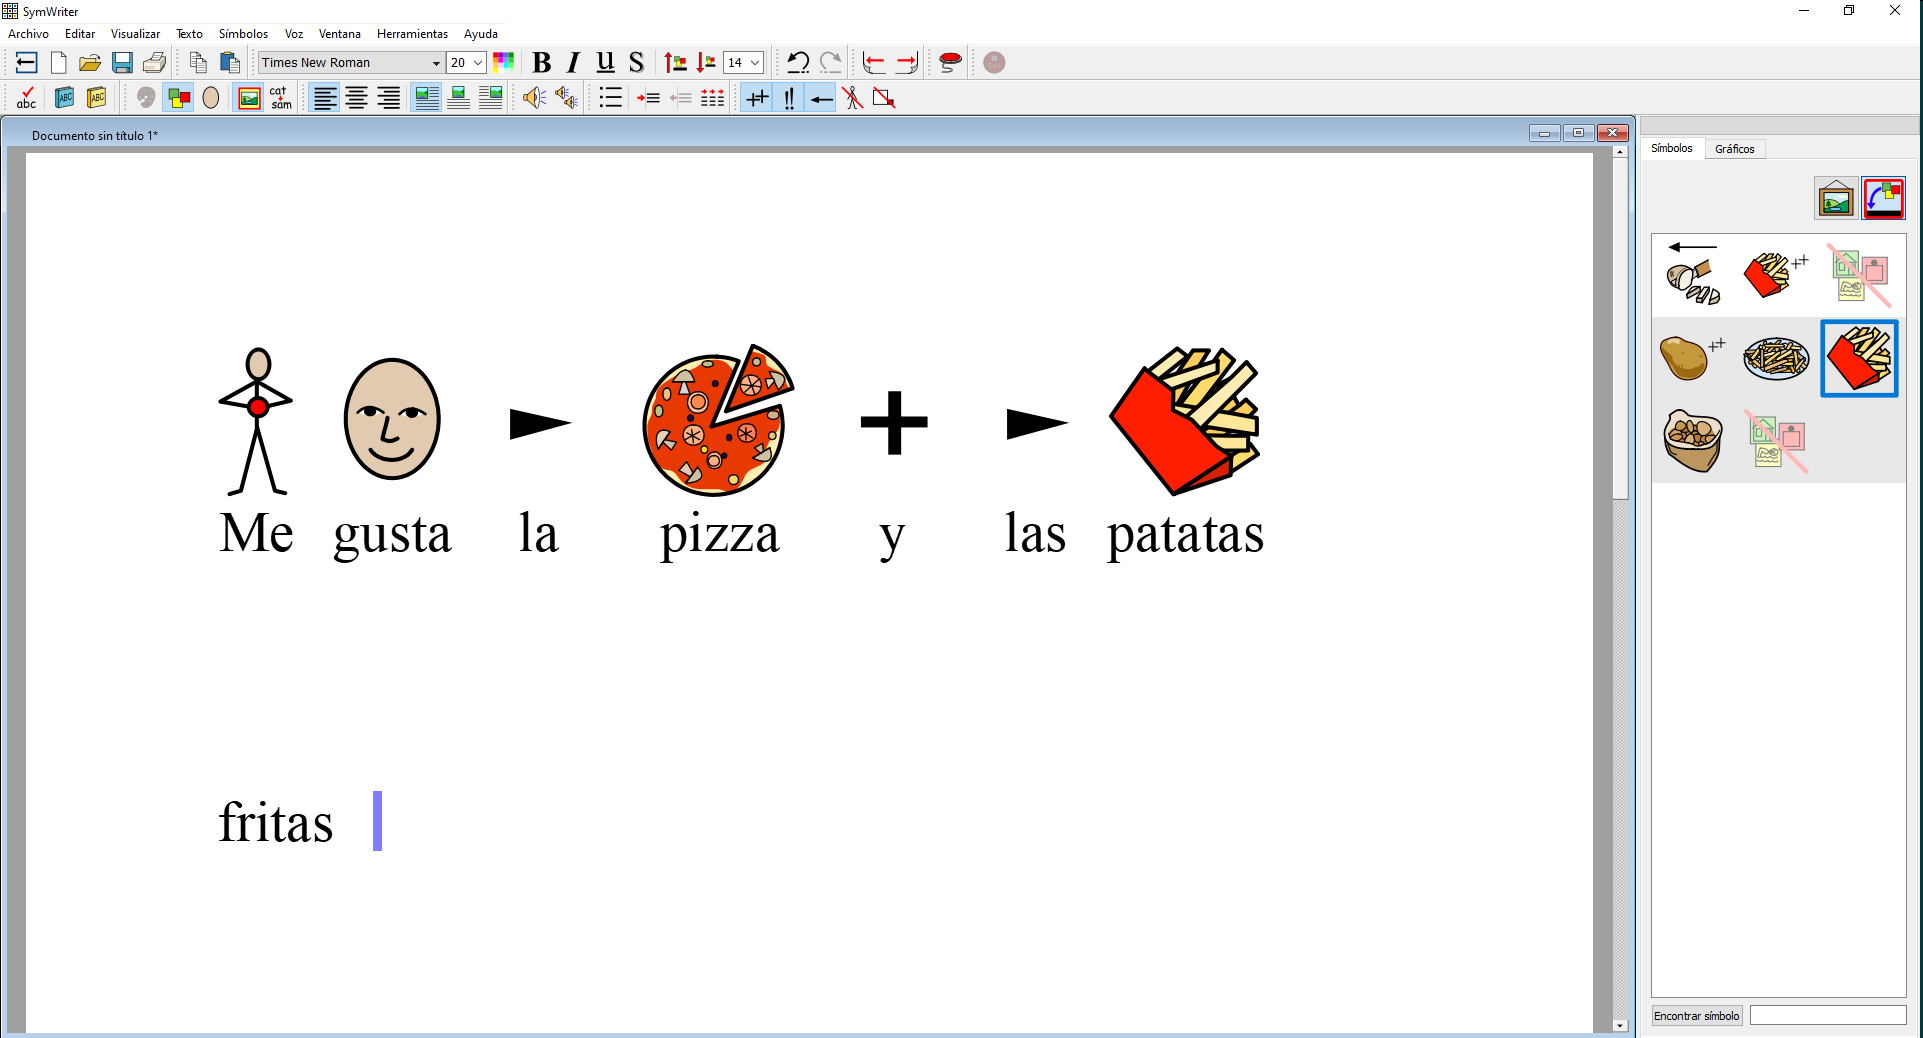
\includegraphics[scale=0.20]{Herramientas_Existentes/SymWriter.png}
    \caption{Interfaz de SymWriter}
    \label{fig:SymWriter}
\end{figure}

\subsection{EducaPlay}
EducaPlay\footnote{\url{https://es.educaplay.com/?lang=es}} es una aplicación web que permite crear actividades interactivas o juegos didácticos. Entre las actividades que se pueden realizar en EducaPlay hay sopas de letras, juegos de memoria, mapas interactivos, ejercicios de relacionar columnas, etc. EducaPlay está pensada, principalmente, para que los alumnos realicen las actividades desde un ordenador o dispositivo móvil, pero permite imprimir las actividades en papel. En la Figura \ref{fig:EducaPlay_Actividad} se muestra una actividad interactiva de EducaPlay y en la Figura \ref{fig:EducaPlay_Impresion} se muestra el formato de impresión de esta actividad.

\begin{figure}[ht!]
    \centering
    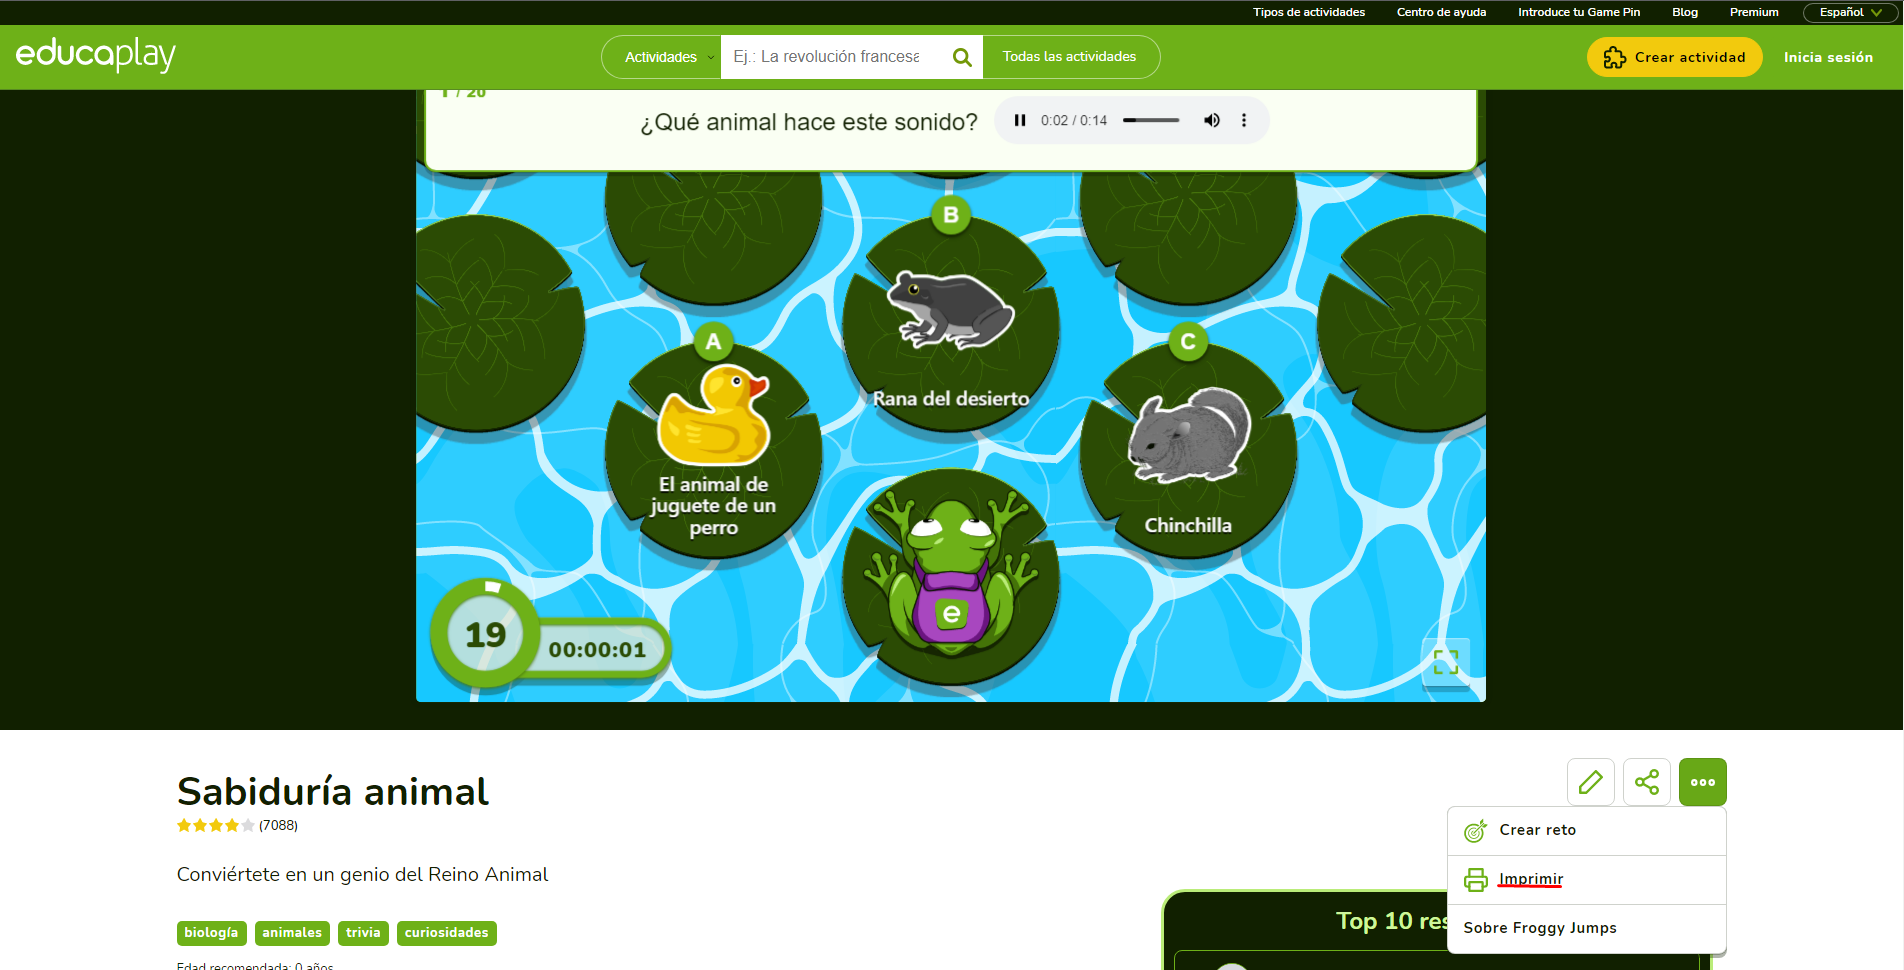
\includegraphics[scale=0.25]{Herramientas_Existentes/EducaPlay_Actividad}
    \caption{Actividad de EducaPlay}
    \label{fig:EducaPlay_Actividad}
\end{figure}

\begin{figure}[ht!]
    \centering
    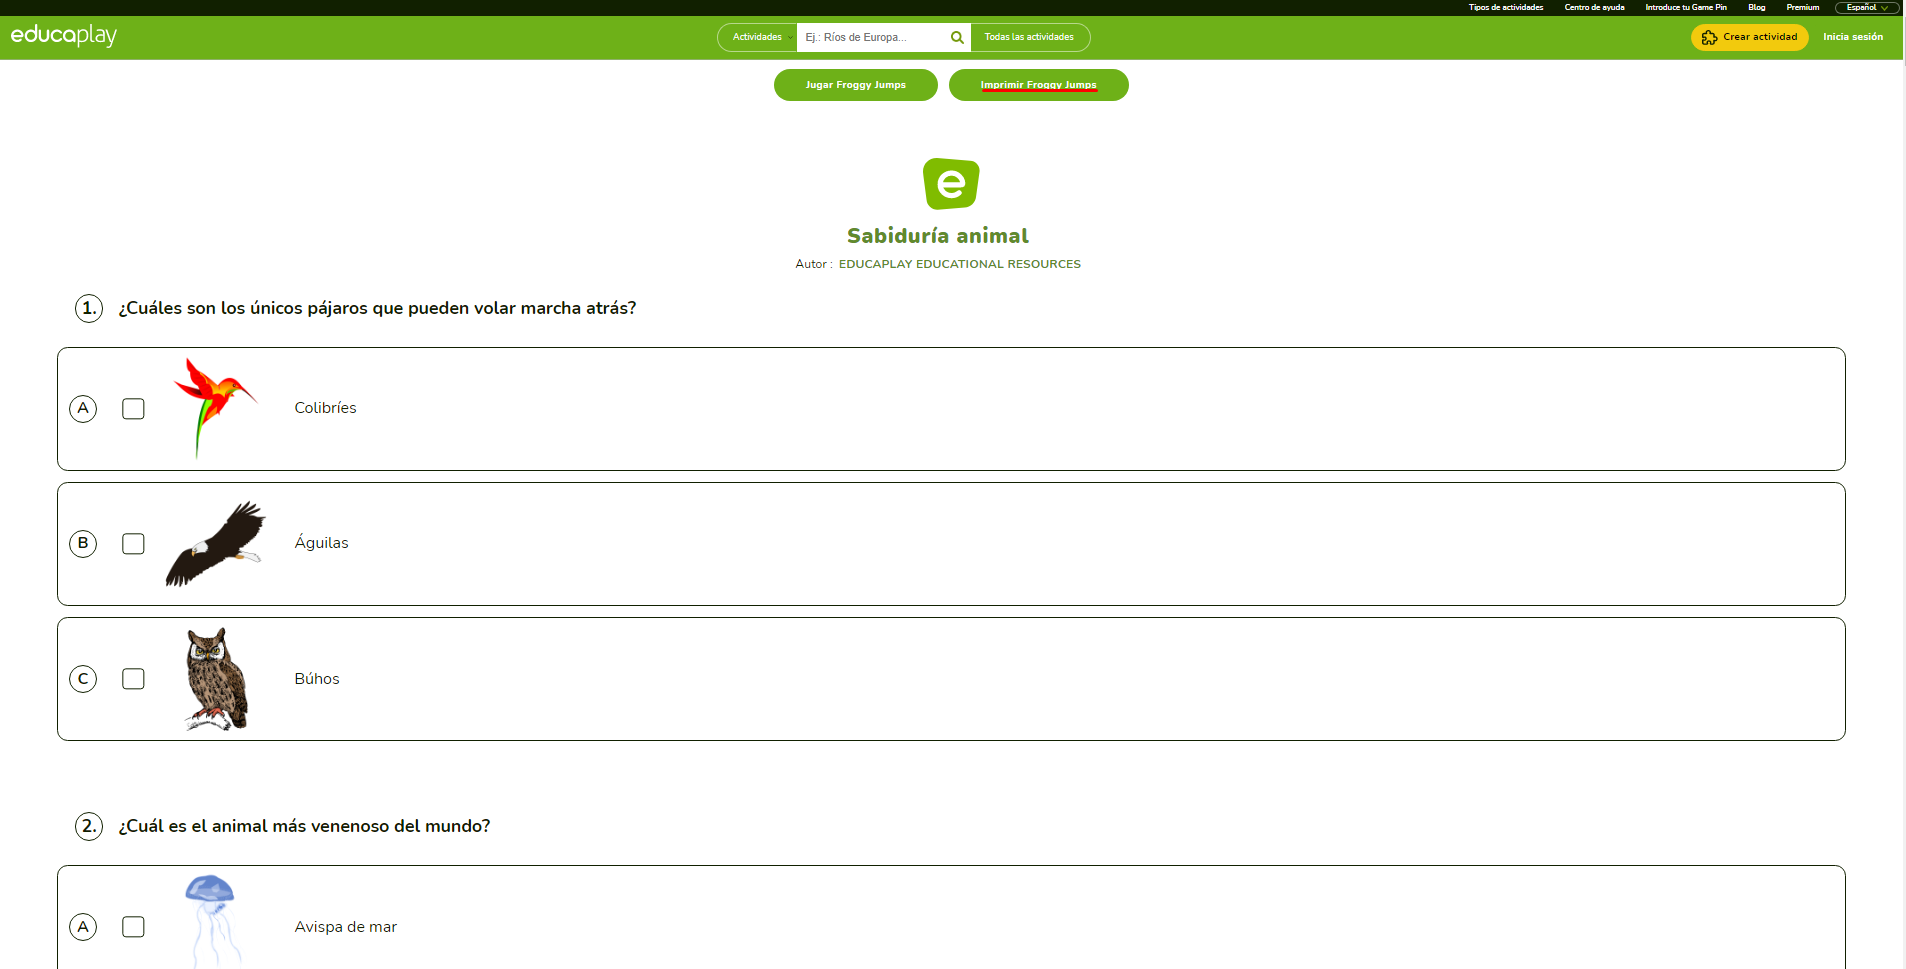
\includegraphics[scale=0.25]{Herramientas_Existentes/EducaPlay_Impresion}
    \caption{Impresión de actividad de EducaPlay}
    \label{fig:EducaPlay_Impresion}
\end{figure}

\subsection{AdaptaMaterialEscolar 1.0}
\label{cap:adaptaMaterial}
La finalidad de AdaptaMaterialEscolar es proporcionar una herramienta para el profesorado con el fin de realizar adaptaciones no significativas a los contenidos de las asignaturas de forma intuitiva, rápida y simple. Actualmente permite realizar las siguientes funciones:
\begin{itemize}
    \item Subir un documento fuente PDF, a partir del cual se puede realizar las adaptaciones, ejercicios, etc.
    \item Buscar pictogramas: Dada una palabra devuelve un pictograma (Figura \ref{Pictogramas}).
    \item Generar ejercicios de completar huecos: Dado un texto se pueden seleccionar las palabras que deben ser sustituidas por espacios en blanco (Figura \ref{Huecos}).
    \item Proporcionar ejercicios de definiciones: Recibe una serie de conceptos a definir y devuelve un ejercicio en base a ellos (Figura \ref{Definiciones}).
    \item Crear ejercicios de desarrollo: Permite crear un enunciado y añadir un cierto número de líneas para la respuesta (Figura \ref{Desarrollo}).
    \item Generar sopas de letras: El usuario introduce las palabras que desea que se pongan en la sopa de letras y el tamaño de la matriz (Figura \ref{Sopa}).
    \item Crear ejercicios de verdadero o falso: Genera una lista con las frases introducidas permitiendo definir cuales son verdaderas o falsas (Figura \ref{VF}).
\end{itemize}

\begin{figure}[ht!]
    \centering
    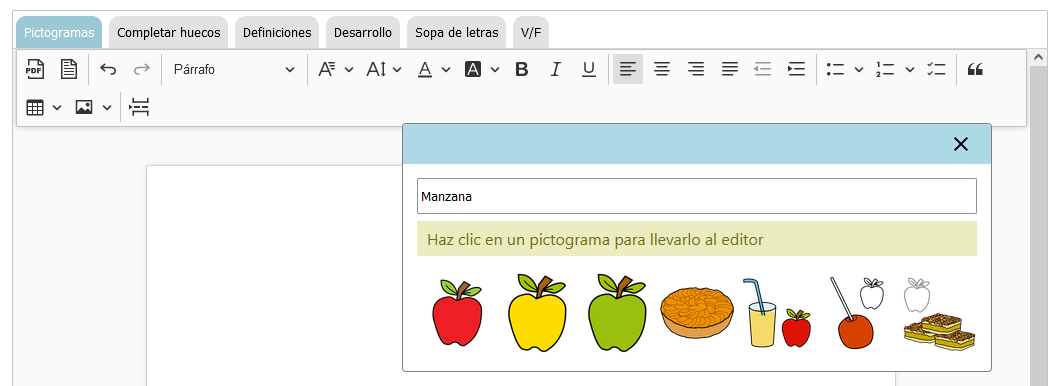
\includegraphics[scale=0.3]{ AdaptaMaterialEscolar/Pictogramas}
    \caption{Busqueda de pictogramas}
    \label{Pictogramas}
\end{figure}
\begin{figure}[ht!]
    \centering
    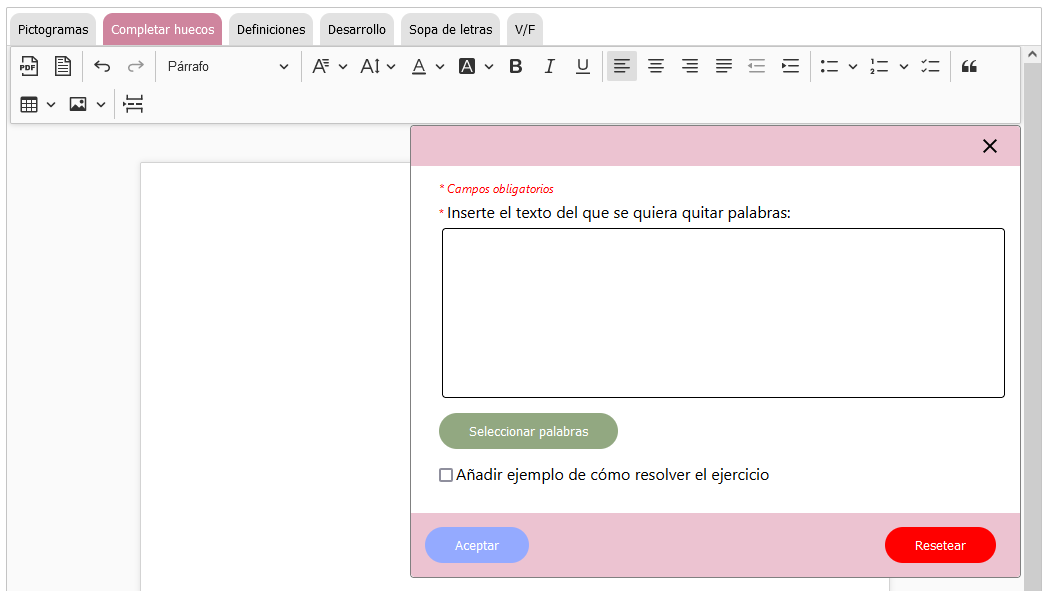
\includegraphics[scale=0.3]{ AdaptaMaterialEscolar/Huecos}
    \caption{Ejercicios de completar huecos}
    \label{Huecos}
\end{figure}
\begin{figure}[ht!]
    \centering
    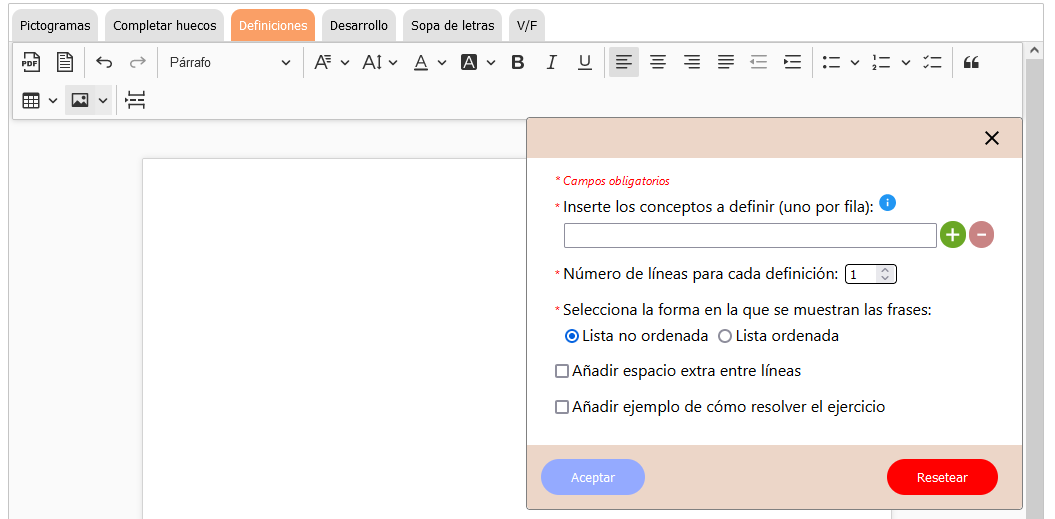
\includegraphics[scale=0.3]{ AdaptaMaterialEscolar/Definiciones}
    \caption{Ejercicios de definiciones}
    \label{Definiciones}
\end{figure}
\begin{figure}[ht!]
    \centering
    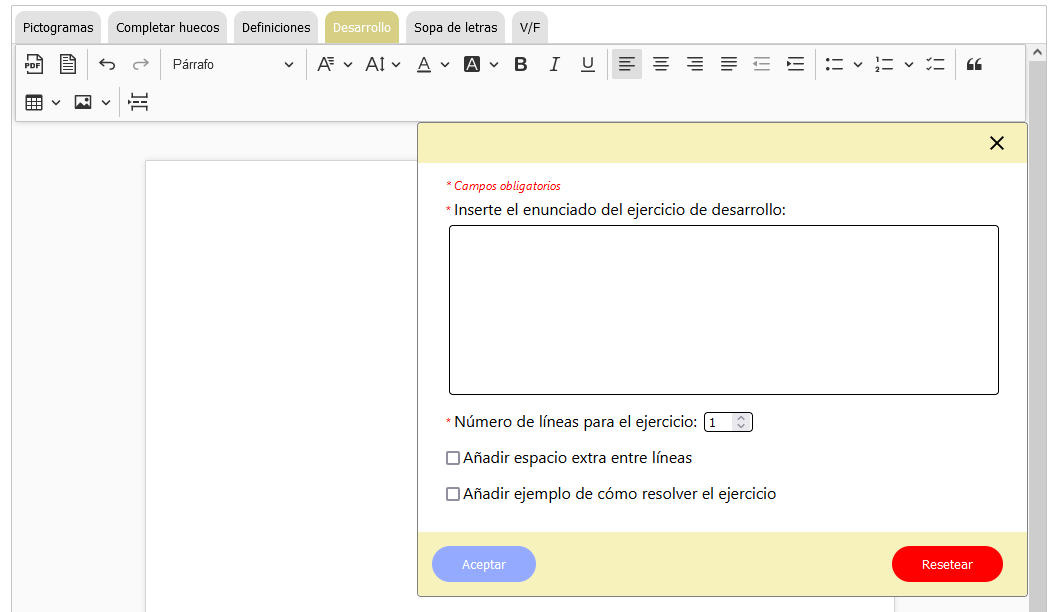
\includegraphics[scale=0.3]{ AdaptaMaterialEscolar/Desarrollo}
    \caption{Ejercicios de desarrollo}
    \label{Desarrollo}
\end{figure}
\begin{figure}[ht!]
    \centering
    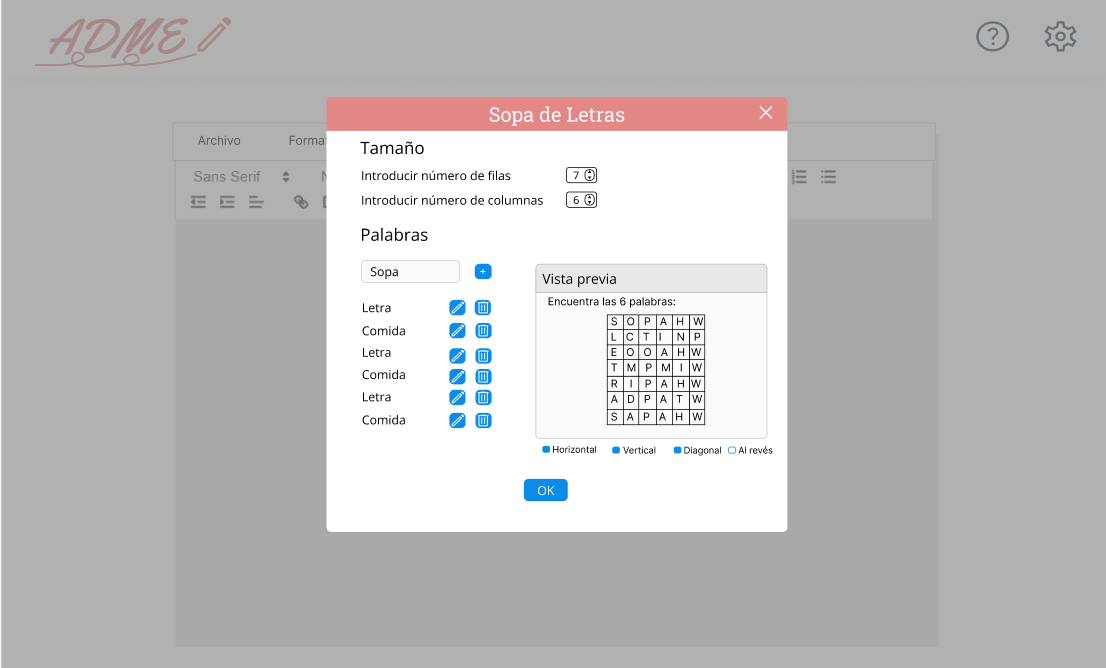
\includegraphics[scale=0.3]{ AdaptaMaterialEscolar/Sopa}
    \caption{Sopas de letras}
    \label{Sopa}
\end{figure}
\begin{figure}[ht!]
    \centering
    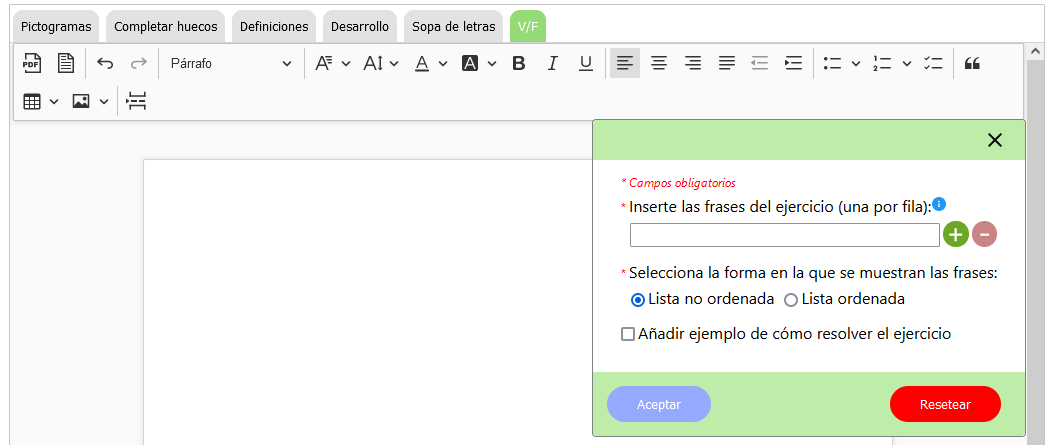
\includegraphics[scale=0.3]{ AdaptaMaterialEscolar/VF}
    \caption{Ejercicios de Verdadero o Falso}
    \label{VF}
\end{figure}
La aplicación se creó siguiendo un Diseño Centrado en el Usuario, para que se adaptase a las necesidades reales de los usuarios finales (los docentes). La captura de requisitos se realizó hablando directamente con el usuario final para poder conocer sus necesidades reales. Para esto se hicieron varias reuniones con 2 profesoras del Aula TEA del IES Maestro Juan de Ávila de Ciudad Real.

Para desarrollar AdaptaMaterialEscolar 1.0 se utilizó React. Para simplificar la gestión del estado de la aplicación, se utilizó Redux. Para el editor de texto de la aplicación se utilizó CKEditor. Por último, para el buscador de pictogramas, se empleó la API de ARASAAC. Esta API permite hacer una petición con un término de búsqueda y devuelve una serie de pictogramas relacionados.

Desde el punto de vista de la arquitectura Figura \ref{arquitecturaADME1}, AdaptaMaterialEscolar 1.0 es una aplicación web \textit{serverless}, es decir, no dispone de \textit{backend}. El \textit{frontend} de esta aplicación se caracteriza por estar basado en una arquitectura orientada a componentes, gracias al uso de la biblioteca de JavaScript React que tiene como objetivo la creación de pequeñas piezas de código independientes, conocidas como componentes, que pueden ser reutilizadas en diferentes partes de la interfaz de usuario. Además, gracias a su enfoque modular, esta arquitectura permite una mayor escalabilidad y mantenibilidad en el desarrollo de aplicaciones web. Sin embargo, como la complejidad de la aplicación puede aumentar significativamente cuando se trabaja con muchos componentes interconectados, se decidió emplear la biblioteca de gestión de estado Redux\footnote{\url{https://redux.js.org/}}. Con Redux, los datos y el estado de los componentes se centralizan en un solo lugar, lo que permite una gestión más eficiente de los mismos y reduce la cantidad de relaciones entre los componentes.

En cuanto al editor de texto utilizado en la aplicación, se optó por CKEditor\footnote{\url{https://ckeditor.com/}}, una solución open source que proporciona una amplia gama de funciones de edición y formateo de texto todo ello para incluir los ejercicios relizados por el profesor.

Además, para implementar la funcionalidad de búsqueda de pictogramas en la aplicación, se decidió utilizar la API de ARASAAC, un repositorio de recursos gráficos diseñado específicamente para personas con necesidades educativas especiales y trastornos del lenguaje. Esta API proporciona una amplia variedad de pictogramas y materiales gráficos, que pueden ser utilizados en aplicaciones educativas y de comunicación alternativa y aumentativa.

También se ha utilizado la biblioteca de \textit{word-search}\footnote{\url{https://www.npmjs.com/package/@blex41/word-search}}, que incluye varias funcionalidades para generar y resolver sopa de letras, como la posibilidad de especificar el tamaño de la cuadrícula, la lista de palabras a buscar, y la orientación en la que se pueden encontrar las palabras. Además, la biblioteca también proporciona opciones para personalizar la apariencia de la sopa de letras, como la fuente, el color y el fondo del la sopa de letras..

\begin{figure}[ht!]
  \centering
  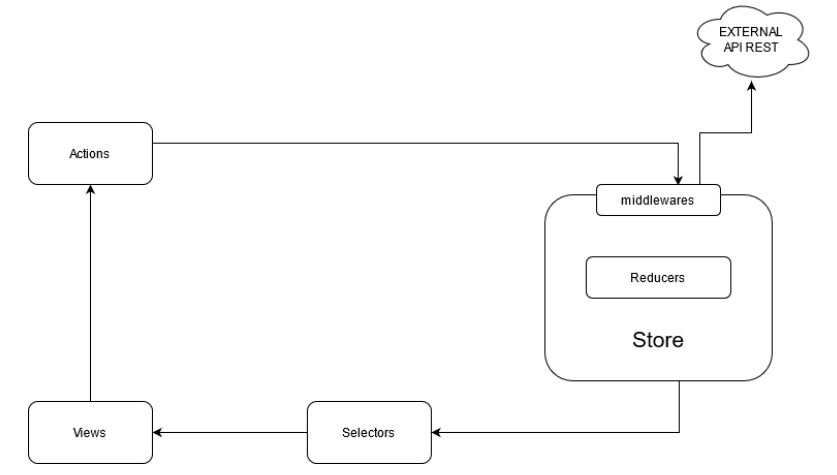
\includegraphics[width=15cm]{Arquitectura/ArquitecturaADME1.PNG}
  \caption{Arquitectura de AdaptaMaterialEscolar 1.0.
  }
  \label{arquitecturaADME1}
\end{figure}


Finalmente la aplicación fue evaluada por los usuarios finales, con el objetivo de descubrir si la aplicación es, en cuanto a la adaptación curricular no significativa, realmente útil para los profesores y si les ayudaba a resolver sus problemas. Para esto se creó un examen de Ciencias Naturales adaptado usando AdaptaMaterialEscolar 1.0. Luego, se replicó este examen con los profesores para mostrarles cómo se usaría la herramienta en situaciones reales. Después de esta demostración, se les hizo una encuesta a los profesores para que pudieran dar su opinión y feedback. Este cuestionario tenía preguntas sobre usabilidad, diseño, funcionalidades y utilidad real de la aplicación. Además, se pasó a los evaluadores el cuestionario SUS (System Usability Scale), que sirve para medir que tan buena es la usabilidad de un sistema. Esta evaluación de la aplicación se realizó con 6 profesores. Como resultado de la evaluación se llegó a la conclusión de que la aplicación sí resuelve problemas reales que tienen los profesores y que se debería seguir desarrollando. A partir del feedback de los usuarios finales que evaluaron la aplicación, se obtuvo una nueva lista de requisitos a implementar para mejorar la aplicación:

\begin{itemize}
    \item Dado un texto traducirlo a pictogramas.
    \item Introducir cuadrícula para ejercicios de matemáticas.
    \item Poder añadir doble pauta, en vez de renglones de una línea, para determinar el tamaño de letra del alumno.
    \item Añadir una herramienta para recortar imágenes.
    \item Añadir encabezado con el nombre del centro educativo, asignatura y nombre del alumno.
    \item Permitir añadir espacio para dibujar en los ejercicios.
    \item Permitir ejercicios de cálculo con fórmulas con huecos que puedan ser rellenados por el alumno.
    \item Enumerar ejercicios automáticamente.
    \item Añadir una fuente de texto parecida a la que suelen aprender la mayoría de los alumnos cuando empiezan a escribir.
\end{itemize}

% TODO: Buscar herramientas de unir conceptos con flechas, generar resumenes...
\subsection{Conclusiones}
Tras investigar las herramientas existentes que tratan de facilitar las adaptaciones curriculares, hemos llegado a la conclusión de que no existen muchas herramientas con este objetivo y, por lo general, las herramientas que hay se centran solo en un tipo de adaptación. Debido a lo anterior se creó AdaptaMaterialEscolar 1.0 con la idea de ofecer una amplia gama de ejercicios para facilitar la adaptación curricular no significativa. Analizando AdaptaMaterialEscolar 1.0 encontramos varias funcionalidades sin implementar y nuevas propuestas descritas por los usuarios finales los cuales estaban bastente interesados en la aplicación. Es por esto por lo que se decidió crear AdaptaMaterialEscolar 2.0.
% TODO: Aportar ejemplos